\subsection{Problem 2a}

\begin{figure}[h]
    \centering
    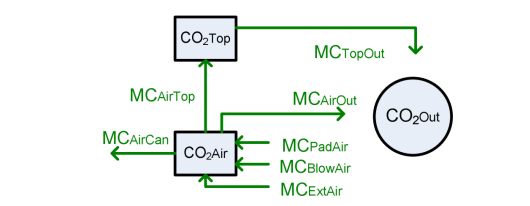
\includegraphics[width = 5in, height = 2in]{Code/Pic/figure.PNG}
    \caption{The $CO_2$ flow inside and outside a greenhouse}
    \label{fig:my_label}
\end{figure}

\begin{figure}[h]
    \centering
    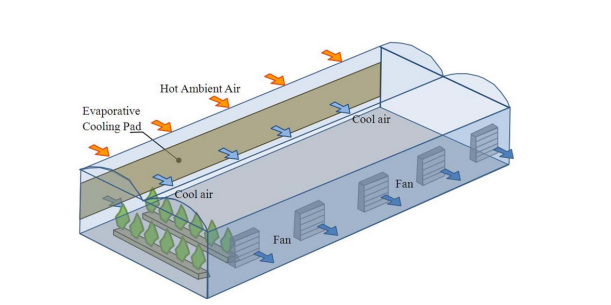
\includegraphics[width = 5in, height = 2in]{Code/Pic/green.png}
    \caption{The movement of $CO_2$ through the pad system and fan system.}
    \label{fig:my_label}
\end{figure}

The two main equation to calculate the $CO_2$ concentration in the lower and upper compartments is

\begin{equation}
\begin{array}{r}
cap_{CO_{2} Air} \Dot{CO_{2Air}}=MC_{BlowAir}+MC_{ExtAir}+MC_{PadAir} \\
-MC_{AirCan}-MC_{AirTop}-MC_{AirOut}
\end{array}
\end{equation}

\begin{equation}
\operatorname{cap}_{\mathrm{CO}_{2} \mathrm{Top}} \Dot{{CO}_{2} \mathrm{Top}}=M C_{\text {AirTop }}-M C_{\text {TopOut }}
\end{equation}

First, the equation to calculate $MC_{\text {BlowAir }}$ is: 

\begin{equation}
M C_{\text {BlowAir }}=\frac{\eta_{\text {Heat } C O_{2}} U_{\text {Blow }} P_{\text {Blow }}}{A_{Flr}}
\end{equation}

Similarly, the amount of $CO_2$ that is pumped into the greenhouse by the third party that supplies $CO_2$ is given by
\begin{equation}
M C_{\text {ExtAir }}=\frac{U_{ExtCO_{2}} * \phi_{ExtCO_{2}}}{A_{Fl r}}
\end{equation}

The following formula is used to calculate $M C_{\text {PadAir }}$:

\begin{equation}
M C_{\text {PadAir }}=f_{\text {Pad }}\left(C O_{2 O u t}-C O_{2 \text { Air }}\right)=\frac{U_{P a d} \phi_{\text {Pad }}}{A_{F l r}}\left(C O_{2 O u t}-C O_{2 \text { Air }}\right)
\end{equation}

The net flux of $CO_2$ from the lower compartment to the upper compartment of the greenhouse is more complicated and it depends on the difference in temperature and air density between the two compartments.
\begin{equation}
MC_{\text{AirTop }}=f_{ThScr}\left(CO_{2} \text {Air}-CO_{2 \text {Top}}\right)
\end{equation}
with $f_{ThScr}$ being:

\begin{equation}
f_{ThScr}=U_{ThScr}K_{ThScr}\left|T_{Air}-T_{Top}\right|^{\frac{2}{3}}+\left(1-U_{ThScr}\right)\left[\frac{g\left(1-U_{ThScr}\right)}{2 \rho_{Air}^{Mean}}\left|\rho_{Air}-\rho_{Top}\right|\right]^{\frac{1}{2}}
\end{equation}

Similarly, for the net $C0_2$ flux from the inside to the outside of the greenhouse, let consider the following formula:

\begin{equation}
MC_{\text {AirOut}}=\left(f_{\text {Ventside }}+f_{\text {VentForced }}\right)\left(CO_{2 \text {Air}}-CO_{2Out}\right)
\end{equation}

To generalize the model for many different types of greenhouses, the following general formula $f_{VentRoofSide}$ $(ms^{-1})$ is used to set the formula for $f_{VentSize}$

\begin{equation}
\begin{array}{r}
f_{\text{VentRoofSide}}=\frac{C_{d}}{A_{\text{Flr }}}\left[\frac{U_{\text {Roof }}^{2} U_{\text{Side }}^{2} A_{\text {Roof }}^{2} A_{\text {Side }}^{2}}{U_{\text {Roof}}^{2} A_{\text {Roof }}^{2}+U_{\text {Side }}^{2} A_{\text {Side }}^{2}} \cdot \frac{2 g h_{\text {SideRoof }}\left(T_{\text {Air }}-T_{\text {Out}}\right)}{T_{\text {Air}}^{\text {Mean }}}\right. \\
\left.+\left(\frac{U_{\text {Roof }} A_{\text {Roof }}+U_{\text {Side }} A_{\text {Side }}}{2}\right)^{2} C_{w} v_{\text {Wind }}^{2}\right]^{\frac{1}{2}}
\end{array}
\end{equation}

In addition, this topic also explores insect screens on ventilation openings and ventilators and
the leakage coefficient of the greenhouse. In the presence of an insect screen, the movement speed
of the air currents through the ventilation areas will be reduced by a factor
\begin{equation}
\eta_{\text {Ins} Scr}=\zeta_{\text {Ins}Scr}\left(2-\zeta_{\text {Ins} Scr}\right)
\end{equation}
where $\eta_{InsScr}$ is the porosity (dimensionless), which is the ratio of the area of the holes in the
screen to the total area of the screen. Given the leakage coefficient $c_{leakage}$ , which depends on the
greenhouse type and is dimensionless, the air-exchange rate is added an amount of approximately
50\% of the leakage rate


\begin{equation}
f_{\text {leakage }}=\left\{\begin{array}{ll}
0.25 \cdot c_{\text {leakage }}, & v_{\text {Wind }}<0.25 \\
v_{\text {Wind }} \cdot c_{\text {leakage }}, & v_{\text {Wind }} \geq 0.25
\end{array}\right.
\end{equation}

The $f_{VentSide}$ is given by the following

\begin{equation}
f_{\text {Ventside }}=\left\{\begin{array}{l}
\eta_{\text {Ins } S c r} f_{Ventside}^{\prime \prime}+0.5 f_{leakage}   ,\eta{side} \geq \eta_{Side_Thr}\\
\eta_{\text {Ins } S c r}\left[U_{\text {ThScr }} f_{\text {Ventside }}^{\prime \prime}\right. \\
\left.+\left(1-U_{\text {ThScr }}\right) f_{\text {Vent Roof Side }} \eta_{\text {Side }}\right]+0.5 f_{\text {leakage}}, \eta{side}< \eta_{Side_Thr}
\end{array}\right.
\end{equation}

The flux $f_{VentForced}$ by the fan system inside the greenhouse is calculated as follows

\begin{equation}
f_{{VentForced}}=\frac{\eta_{\text{InsScr}} U_{VentForced} \phi_{VentForced}}{A_{Flr}}
\end{equation}


Similarly to $MC_{AirOut}$, the net CO2 flux from the greenhouse to outside the greenhouse
through the roof openings is calculated by using the formula

\begin{equation}
M C_{TopOut}=f_{VentRoof}\left(CO_{2Top}-CO_{2Out}\right)
\end{equation}

where $f_{VentRoof}$ is the flux rate through the roof openings and is given by

\begin{equation}
f_{\text {VentRoof}}=\left\{\begin{array}{l}
\eta_{\text {Ins}Scr} f_{\text {VentRoof}}^{\prime \prime}+0.5 f_{\text {leakage}},\eta{roof} \geq \eta_{Roof_Thr}\\
\eta_{\text {Ins}Scr}\left[U_{\text {ThScr}} f_{\text {VentRoof}}^{\prime \prime}\right. \\
\left.+\left(1-U_{\text {ThScr}}\right) f_{VentRoofSide} \eta_{\text {Side }}\right]+0.5 f_{\text {leakage}}, \eta_{Roof}<\eta_{Side_Thr}
\end{array}\right.
\end{equation}

with

\begin{equation}
f_{VentRoof}^{\prime\prime}=\frac{C_{d}U_{Roof}A_{Roof}}{2A_{Flr}}\left[\frac{gh_{Vent}\left(T_{Air}-T_{Out}\right)}{2 T_Air}^{\text {Mean}}}+C_{w} v_{Wind}^{2}\right]^{\frac{1}{2}}
\end{equation}

Finally, we need to describe the amount of CO2 that is absorbed into the leaves due to photosynthesis.

\begin{equation}
M C_{\text {AirCan }}=M_{C H_{2} O} h_{C_{B u f}}(P-R)
\end{equation}
with

\begin{equation}
h_{C_{Buf}}=\left\{\begin{array}{ll}
0, & C_{Buf}>C_{Buf}^{Max} \\
1, & C_{Buf} \leq C_{Buf}^{Max}
\end{array}\right.
\end{equation}

. Usually, the
respiration rate $R$ is negligible compared to the photosynthetic rate $P$ and can be omitted or calculated
as about 1\% of the photosynthetic rate. To simplify the assignment, $h_{C_{Buf}}$ will always have a value of 1, meaning that $C_{Buf}$ will have
no effect on the CO2 fluctuation.

We will use Equation (9.10) and relevant
ones in reference [Van11] to solve Equation (18) in this exercise with assumption that $PAR_{Can}$ is a constant

\subsection{Problem 2b}
We use data for coefficients given by "A methodology for model-based greenhouse design" by Vanthoor, , C. Stanghellini,  E.J. van Henten and P.H.B. de Visser as well as "A model-based greenhouse design method" by Bram Vanthoor.
The data for $CO_{2_{Air}}$ and  $CO_{2_{Top}}$ came from https://github.com/CEAOD/Data
\begin{figure}[h]
\centering
    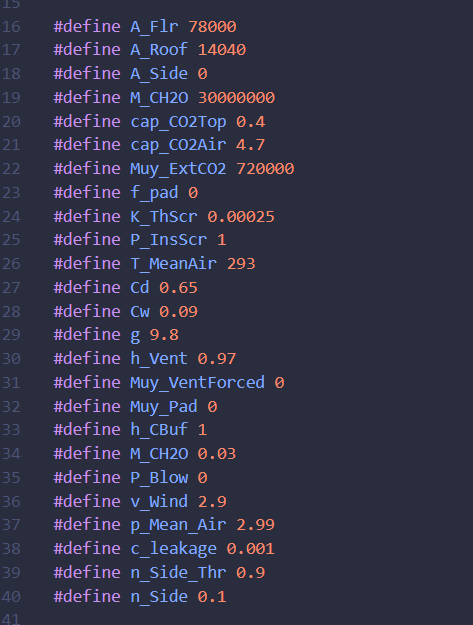
\includegraphics[width = 4in, height = 4in]{Code/Pic/constant.png}
    \caption{Declaring constants}
    \label{fig:my_label}
\end{figure}


We have a function named doublerand used to randomize the control value in the range [0,1]

\begin{figure}[h]
\centering
    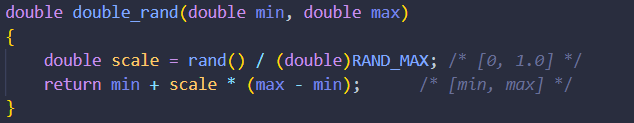
\includegraphics[width = 5.5in, height = 1.5in]{Code/Pic/random.png}
    \caption{Randomize function}
    \label{fig:my_label}
\end{figure}

The function \text{read\_record} is used to read the .csv input file

After that, we simply write the code using all the formulas mentioned in problem a of exercise 2

\begin{figure}[h]
\centering
    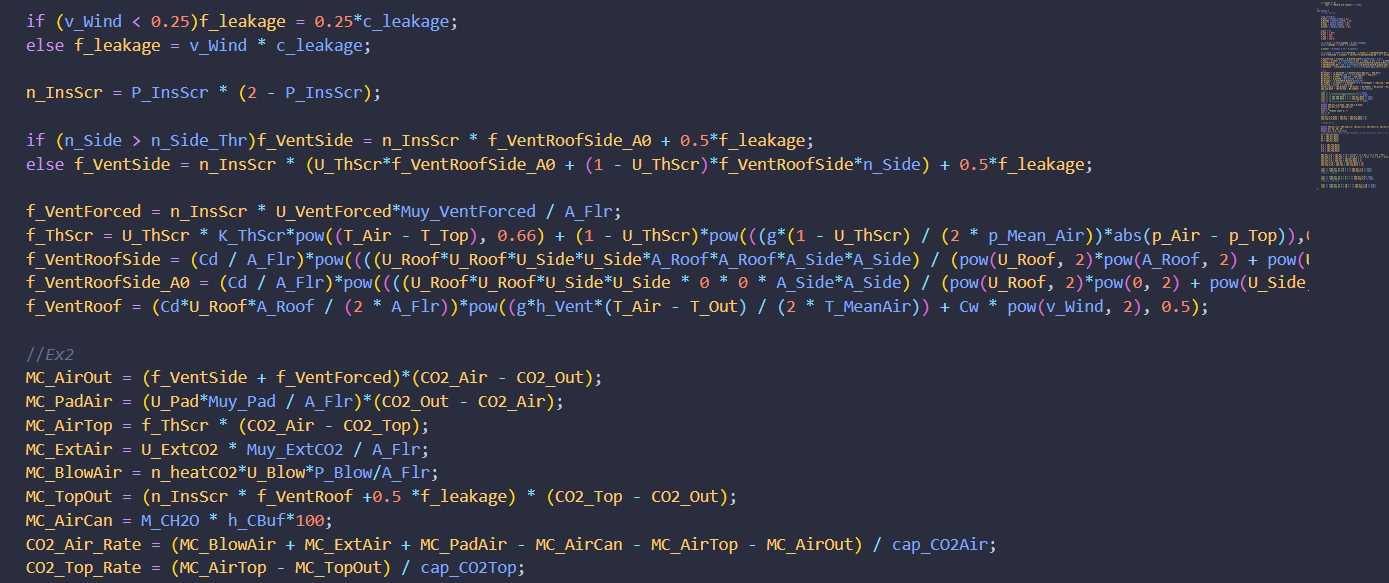
\includegraphics[width = 4in, height = 3in]{Code/Pic/ex2_code.png}
    \caption{Main code}
    \label{fig:my_label}
\end{figure}








